\RequirePackage{shellesc}
\documentclass[a4paper]{article}
\usepackage[document]{ragged2e}
\usepackage{fontspec}
\usepackage{geometry}
\usepackage{titlesec}
\usepackage{graphicx}
\usepackage{float}
\usepackage{minted}
\usepackage{enumitem}
\usepackage{indentfirst}
\usepackage[Export]{adjustbox} % Used to constrain images to a maximum size
\usepackage[font=large]{caption}
\geometry{left=2cm}
\geometry{right=2cm}
\geometry{top=2cm}
\geometry{bottom=2cm}
\setmainfont{Liberation Serif}
\setmonofont[Scale=0.7]{Hack}
\titlelabel{\thetitle. }
\renewcommand{\tablename}{Таблица}
\renewcommand{\figurename}{Рисунок}
\counterwithin{table}{section}
\counterwithin{figure}{section}
\captionsetup{justification=raggedright,singlelinecheck=false}
\renewcommand\large{\fontsize{14}{16}\selectfont}
\renewcommand{\theFancyVerbLine}{\textbf{\arabic{FancyVerbLine}}}
\sloppy

\setminted{
  linenos,
  breaklines,
  breakanywhere,
  breaksymbolleft=,
  fontsize=\fontsize{12}{12}\selectfont,
  numbersep=5pt,
}
\usemintedstyle{emacs}

\graphicspath{ {../4/pics/} }

\begin{document}
  \fontsize{14}{16}\selectfont

  \begin{titlepage}
    \begin{minipage}{0.2\textwidth}
      
\includegraphics[scale=0.4]{logo}
    \end{minipage}
    \begin{minipage}{0.7\textwidth}\centering
      \fontsize{10}{12}\selectfont
      \textbf{
        Федеральное государственное бюджетное образовательное учреждение \\
        высшего профессионального образования \\
        «Московский государственный технический университет имени Н.Э. Баумана» \\
        (МГТУ им. Н.Э. Баумана)
      }
    \end{minipage}

    \vspace{5cm}
    \centering
    \fontsize{16}{20}\textbf{
      Лабораторная работа №5 \\
      по курсу «Методы машинного обучения» \\
    }

    \vspace{5cm}
    \begin{flushright}
    Выполнил \\
    студент группы ИУ5-22М \\
    XXXX \\
    \end{flushright}
    \vspace*{\fill}
    Москва, 2023
  \end{titlepage}

  \justifying
  \setlength{\parindent}{1.25cm}

  \section{Задание}
  На основе рассмотренного на лекции примера реализуйте следующие алгоритмы:
  \begin{itemize}
    \item SARSA
    \item Q-обучение
    \item Двойное Q-обучение
  \end{itemize}

  \section{Текст программы}
  \inputminted{python}{5.py}

  \section{Экранные формы с примерами выполнения программы}
  \begin{figure}[H]
    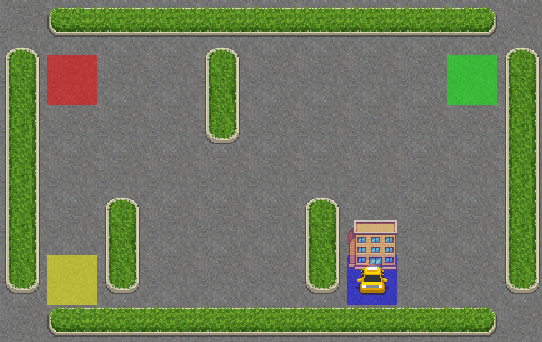
\includegraphics[scale=0.5]{52}
  \end{figure}
  \noindent Q-обучение: eps=0.4, lr=0.1, gamma=0.98, num\_episodes=20000
  \begin{minted}{text}
Вывод Q-матрицы для алгоритма  Q-обучение
[[ 0.          0.          0.          0.          0.          0.        ]
 [ 5.09940217  5.11613495  4.9333549   6.24799219  8.36234335 -3.62258081]
 [10.04299356 11.11574742  9.6393241  11.43318009 13.27445578  2.65833957]
 ...
 [-1.36364673 11.89866367  0.31299649  0.12111493 -2.18307592 -4.64070247]
 [-2.6539698   8.34882836 -2.02398777  0.61115667 -8.4092672  -7.78482003]
 [11.04932363  4.15528476  7.05358754 18.59990519  2.11145862  4.24396103]]
  \end{minted}
  \begin{figure}[H]
    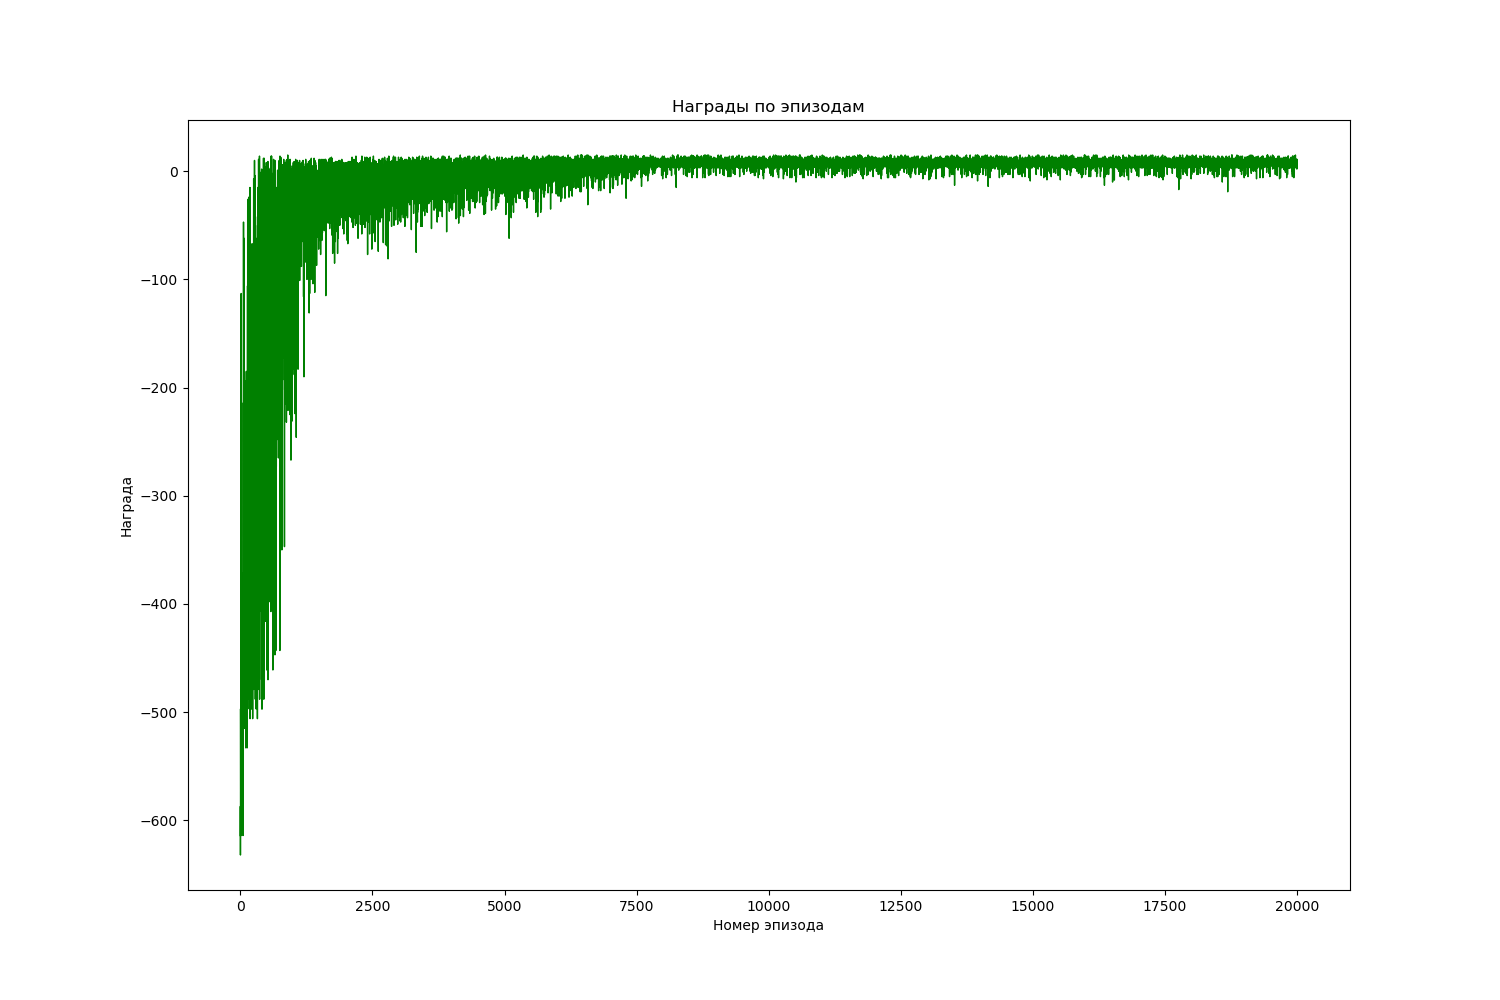
\includegraphics[scale=0.35]{51}
  \end{figure}

  \noindent Двойное Q-обучение: eps=0.4, lr=0.1, gamma=0.98, num\_episodes=20000
  \begin{minted}{text}
Вывод Q-матриц для алгоритма Двойное Q-обучение
Q1
[[ 0.          0.          0.          0.          0.          0.        ]
  [-0.72267154  1.85252442  0.19552651  2.85144428  8.36234335 -6.59195419]
  [ 7.18532871  6.59356075  5.37962679  5.5787384  13.27445578 -4.09009116]
  ...
  [-0.66467311 12.85534519 -1.95425954 -2.31569204 -5.48922472 -4.37459481]
  [-3.22093218 -3.91954695 -3.58949805  1.68910615 -7.61442506 -8.67036163]
  [ 3.79014035  3.88911184  5.13464853 18.25507162  0.68488221  1.74249151]]
Q2
[[ 0.          0.          0.          0.          0.          0.        ]
  [-0.77584626  3.15691246  0.69250749  2.73240034  8.36234335 -5.35095443]
  [ 4.20528463  7.68270196  4.62451724  3.56948691 13.27445578 -1.14602156]
  ...
  [-1.54713418 13.67037706  0.3485602  -0.64388233 -7.43964304 -4.11504528]
  [-4.99805617 -4.01629887 -3.96321961  2.922531   -4.97259003 -3.3258903 ]
  [ 2.08418592  0.94533048  1.13723617 18.48774274 -1.7645767  -0.50591363]]
  \end{minted}
  \begin{figure}[H]
    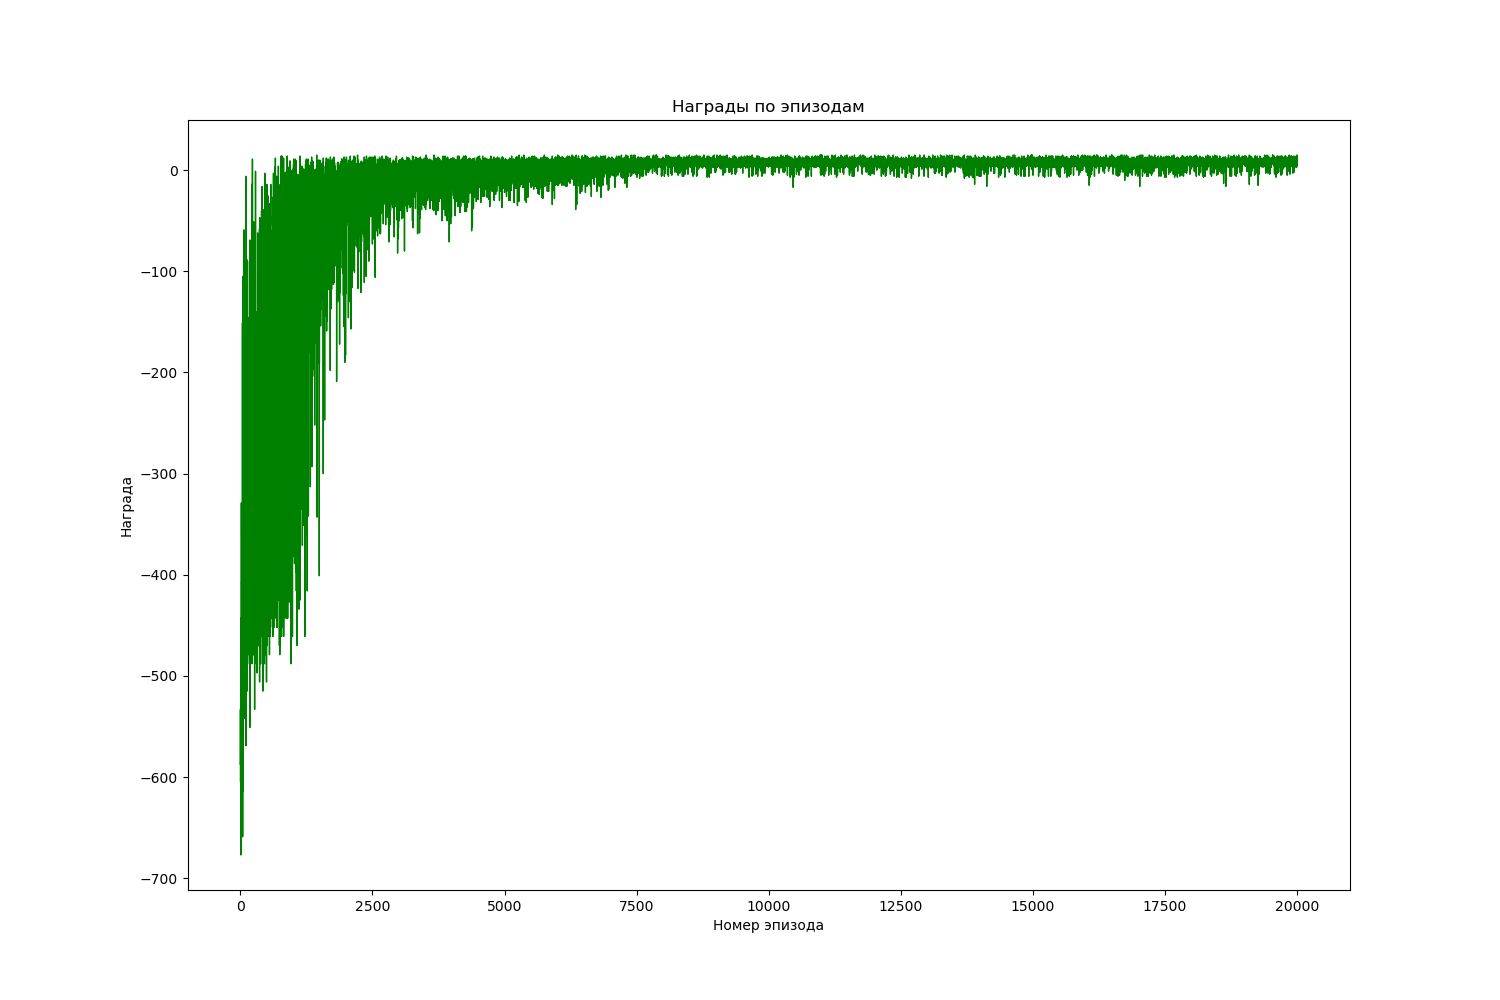
\includegraphics[scale=0.35]{53}
  \end{figure}

  \noindent SARSA: eps=0.4, lr=0.1, gamma=0.98, num\_episodes=20000
  \begin{minted}{text}
Вывод Q-матрицы для алгоритма  SARSA
[[  0.           0.           0.           0.           0.
    0.        ]
 [ -8.66665356  -5.19580592  -3.60445722  -2.81367279   7.94897997
   -10.02695965]
 [ -0.13055387  -0.3346179    0.34120444   5.34029633  13.19676101
    -3.77660174]
  ...
 [ -0.65210655  10.87574541  -2.27322581  -2.06382686  -7.35227183
    -4.84737165]
 [ -8.37712909  -4.26957472  -8.15637214  -7.89962417 -14.04817395
   -13.32447119]
 [  8.81479907   7.35859204   6.83248527  18.47612868  -0.1078542
     0.98660318]]
  \end{minted}
  \begin{figure}[H]
    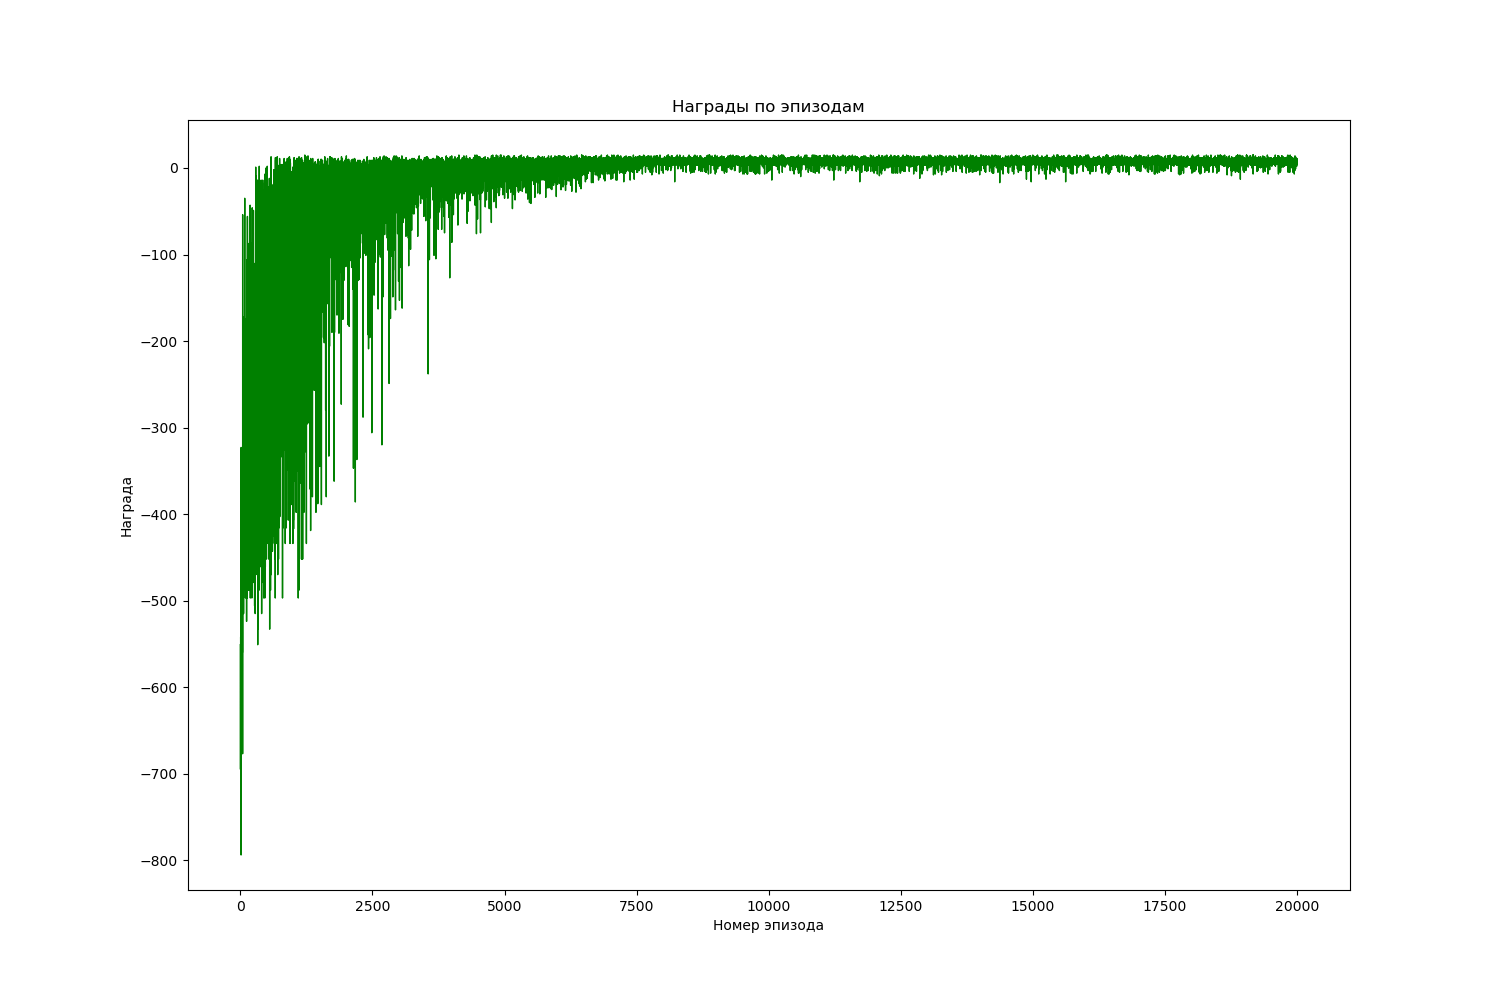
\includegraphics[scale=0.35]{54}
  \end{figure}
  \pagebreak

  \section{Вывод}
  На параметрах по умолчанию быстрее всего сходится Q-обучение.
  Gamma подобрана удачно, крупные изменения значения делают результат хуже.
  Быстрая сходимость получается на eps = 0.1:
  \begin{figure}[H]
    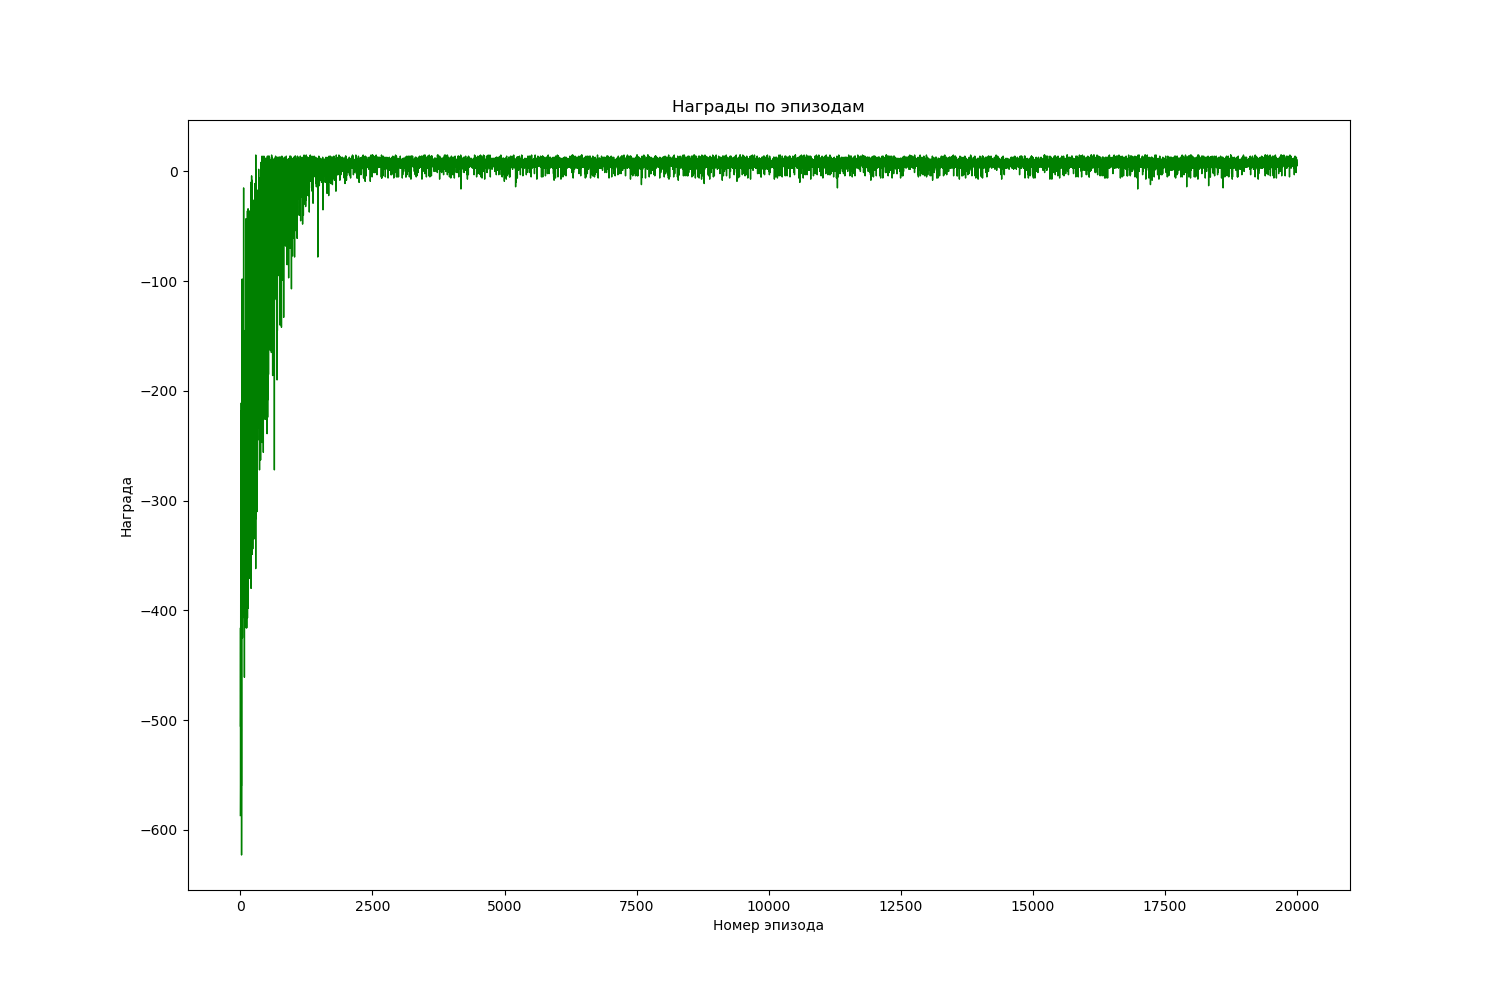
\includegraphics[scale=0.35]{55}
  \end{figure}

  SARSA также быстрее сходится при уменьшении eps.
  Learning rate и gamma подобраны удачно.
\end{document}
